\documentclass[11pt, a4paper]{scrartcl}
\usepackage[ngerman]{babel}
%\usepackage[T1]{fontenc}
\usepackage[utf8]{inputenc}
\usepackage{amsmath}
\usepackage{amssymb}
\usepackage{amsthm}
\usepackage{graphicx}
\usepackage{listings}
\usepackage{booktabs}
\usepackage{float}
\usepackage{pdfpages}
%
\begin{document}
\lstset{basicstyle=\small,
		 inputencoding=latin1,
		stringstyle=\ttfamily,
		identifierstyle=,
		showstringspaces=false,
		language=c,
		frame=trBL}
%
\subsection*{TI III WS 2013, Fr. 12-14}
\section*{Lösung Übungsblatt 4}
\textbf{Christoph van Heteren-Frese (Matr.-Nr.: 4465677), Julien  Stengel } \\%(Matr.-Nr.: 4567553)}\\
Tutor: Ruhland, eingereicht am \today\\
\hrule
%
\section*{Aufgabe 3: Speicherzuteilung}
Aus der manpage von \texttt{malloc}:
\begin{quotation}
\noindent
\textit{void *malloc(size\_t size);\\
...\\
Malloc() allocates  size  bytes and returns a pointer to the allocated memory.	The memory is not cleared.}
\end{quotation}
Somit versucht der Aufruf von\texttt{ malloc(1000000000000)} genau  $10^{12}$ Bytes, also 1 Terrabyte bereitzustellen.
Dies gelingt nicht ein einziges Mal!	

Der größtmögliche Speicherbereich, der mit \texttt{malloc()} angefordert werden kann, hängt sowohl vom physikalischen Speicher als auch dem verwendeten Betriebssystem ab. Theoretisch wir er vom verwendetet typ \texttt{size\_t} limitiert, der selbst durch 4 Byte repräsentiert wird und somit also maximal den Wert $2^{32}-1$ = 4.294.967.295 darstellen kann (ohne Vorzeichen). malloc(1000000000000) verursacht beim compilieren dementsprechend die Warnung
\begin{quote}
\textit{mal.c:5:3: Warnung: Große Ganzzahl implizit auf vorzeichenlosen Typen abgeschnitten [-Woverflow]}
\end{quote}
\section*{Aufgabe 4}
\subsection*{a)} 
\lstinputlisting{../u4_4.c}
\subsection*{b)}
Es gibt drei Modi eine Datei zu öffnen: \texttt{r}, \texttt{w}, \texttt{a}. Abhängig vom verwendeten Compiler und c-Standart (c89/c90, c99, c11) ist es notwendig ein \texttt{b} für binary bzw. ein \texttt{t} für text zu ergänzen. 
\begin{figure}[H]
\center
\begin{tabular}{lp{1.9cm}p{10cm}}
\toprule
%&&& \multicolumn{2}{c}{Datei vor Aufruf} \\
\textit{Modus} & Bedeutung & Bemerkung \\%& existent & \textbf{nicht} existent\\
\midrule 
r & read & Öffnet eine Datei um am Anfang beginnend aus ihr zu lesen. Existiert die Datei nicht, bricht die Funktion mit einem Fehler ab. \\ \addlinespace
w & write & Erzeugt eine Datei um in ihr zu schreiben. Existiert die Datei be\-reits, wird der Inhalt zerstört.\\ \addlinespace
a & append & Öffnet eine Datei und fügt an das Ende des Inhalts an.\\ \addlinespace
r+ & read \textit{\mbox{extended}} & Öffnet eine Datei am Anfang beginnend um aus/in ihr zu lesen/schreiben. Existiert die Datei nicht, bricht die Funktion mit einem Fehler ab. \\ \addlinespace
w+ & write \textit{\mbox{extended}} & Erzeugt eine Datei zum lesen/schreiben. Existiert die Datei be\-reits, wird der Inhalt zerstört. \\ \addlinespace
a+ & append \textit{\mbox{extended} }& Öffnet eine Datei zum lesen/schreiben. Exisitiert die Datei bereits, wird an das Ende geschrieben. Andernfalls wird die Datei erzeugt.\\ 
\bottomrule \addlinespace
\end{tabular}
\end{figure}
Des Weiteren kann seit c11  bei den Modi \texttt{w} und \texttt{w+} ein \texttt{x} ergänzt werden. Dies hat zur Folge, das die Funktion abbricht, solle die Datei bereits existieren. Der Inhalt wird somit nicht zerstört.

Damit das Beispielprogramm an das Ende der Ausgabedatei schreibt, ist somit nur Zeile 41 zu ändern:
\begin{quote}
\textit{f2 = fopen(argv[2], ''\textbf{a}t'');}
\end{quote}
\subsection*{c)}
Abhänhig vom System macht dies der Regel macht dies keinen Unterschied. In der manpage zu \texttt{fopen} heisst es:
\begin{quote}
\noindent
 \textit{The mode string can also include the letter 'b' either as a last
       character or as a character between the characters in any of the two-
       character strings described above.  This is strictly for
       compatibility with C89 and has no effect; the 'b' is ignored on all
       POSIX conforming systems, including Linux.  (Other systems may treat
       text files and binary files differently, and adding the 'b' may be a
       good idea if you do I/O to a binary file and expect that your program
       may be ported to non-UNIX environments.)}
\end{quote}
Auf meinem System ist dementsprechend kein Unterschied feststellbar.
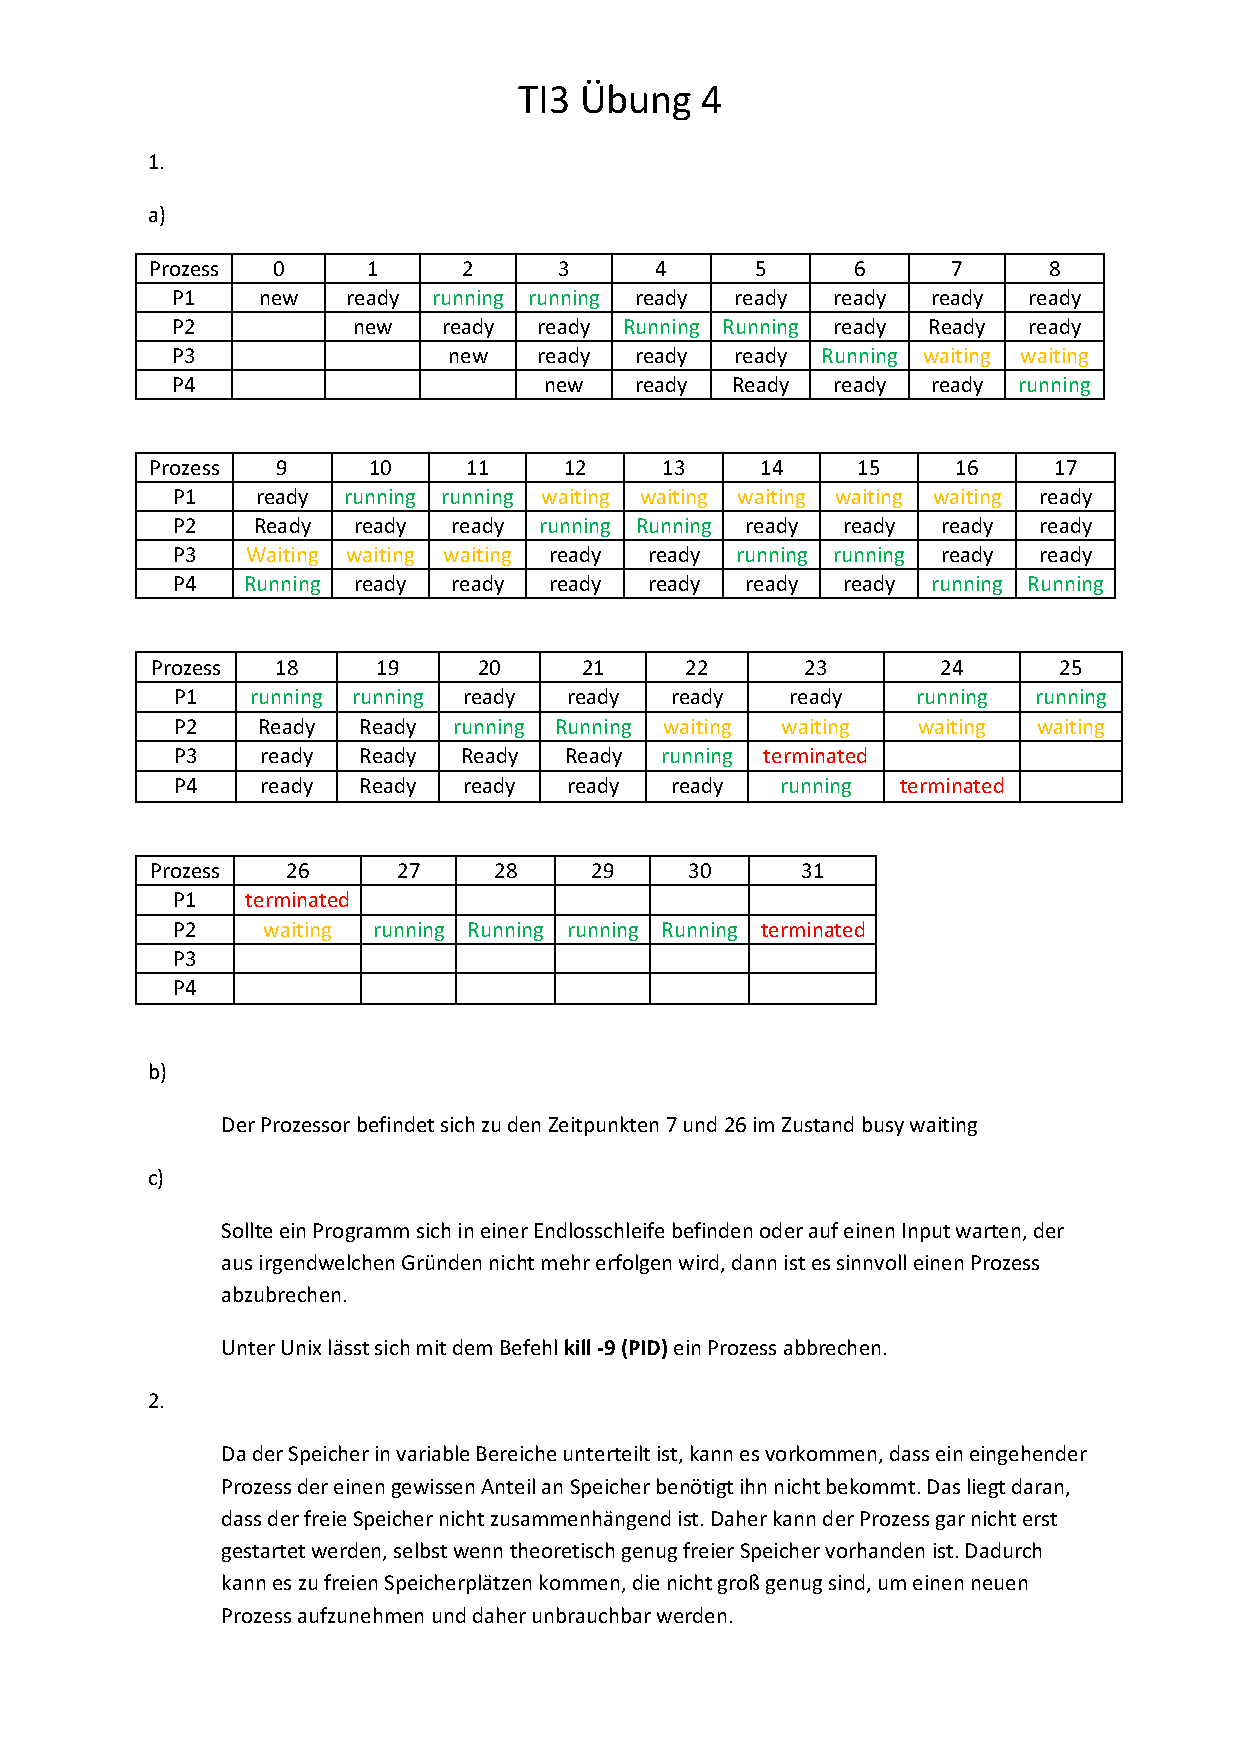
\includepdf[pages={1}]{a1_a2.pdf}
%\includepdf[pages={1}]{blatt2.pdf}

\end{document}
